\documentclass[12pt]{article}

\usepackage{sbc-template}
\usepackage{xcolor}
\usepackage{graphicx,url}

\usepackage[brazil]{babel}   
\usepackage[utf8]{inputenc}  
    
\sloppy

\title{Dropoutless: plataforma colaborativa de predição de evasão}

\author{Laís Pisetta Van Vossen\inst{1}, Maria Teresa Silva Santos\inst{1}, \\Luciana Bolan Frigo\inst{2}, Isabela Gasparini\inst{1} }


\address{Universidade do Estado de Santa Catarina (UDESC)\\
  Joinville, Santa Catarina, Brasil
\nextinstitute
  Universidade Federal de Santa Catarina (UFSC)\\
  Florianópolis, Santa Catarina, Brasil
  \email{\{lais.vossen,maria.santos2805\}@edu.udesc.br}
  \email{ luciana.frigo@ufsc.br,isabela.gasparini@udesc.br }
}

% \author{
% Laís Pisetta Van Vossen\inst{1}, Maria Teresa Silva Santos\inst{1}, \\Luciana Bolan Frigo\inst{2}, Isabela Gasparini\inst{1}
% }

% \address{
% Universidade do Estado de Santa Catarina (UDESC)\\ Joinville, Santa Catarina, Brasil\\
% \nextinstitute
% Universidade Federal de Santa Catarina (UFSC)\\ Florianópolis, Santa Catarina, Brasil
%   \email{\{lais.vossen, maria.santos2805\}@edu.udesc.br, luciana.frigo@ufsc.br, isabela.gasparini@udesc.br}
% }

\begin{document} 

\maketitle

\begin{abstract}
Student dropout is a recurring problem that affects various spheres of society, representing a waste of resources for the state and a decrease in qualified labor for companies. This article proposes a collaborative platform, named Dropoutless, whose aim is to reduce dropout rates in university disciplines by creating co-participative predictive models using AutoML techniques. As a result, the proposed tool allows for greater flexibility in the data used for dropout prediction and promotes the leadership of educators in changing this scenario.
\end{abstract}
     
\begin{resumo} 
A evasão estudantil é um problema recorrente que afeta diversas esferas da sociedade, representando um desperdício de recursos para o Estado e uma queda da mão de obra qualificada para as empresas. Neste artigo é proposta uma plataforma colaborativa, nomeada Dropoutless, cujo objetivo é reduzir a evasão em disciplinas universitárias através da criação de modelos de predição de forma coparticipativa utilizando técnicas de AutoML. Como resultado, a ferramenta proposta permite uma flexibilização nos dados utilizados na predição de evasão e promove o protagonismo dos educadores na mudança desse cenário.
\end{resumo}


\section{Introdução}

% paragrafo 1- evasão (dados de evasão mais recentes em universidades, custo para o estado, etc)

% parágrafo 2 - como diversos trabalhos tem tentando prever evasão em diversos contextos

% parágrafo 3 - a ferramenta proposta

% parágrafo 4 - sobre AutoML

% parágrafo 5 - como o trabalho está dividido


A redução das taxas de evasão em cursos do ensino superior é uma das metas mais desafiadoras para as universidades. Iniciativas como o Programa de Apoio a Planos de Reestruturação e Expansão das Universidades Federais (Reuni) tem como um de seus objetivos o combate a evasão como forma de diminuir as desigualdades sociais no país\footnote{http://reuni.mec.gov.br/o-que-e-o-reuni}. 

Para o Estado, a evasão representa um desperdício de recursos, com a estrutura acadêmica sendo subutilizada com a saída de estudantes que ela poderia comportar. Além disso, o abandono dos estudos pode ser visto como um indicativo de falhas ou ineficiência no processo de ensino \cite{gilioli:2016}. Este fenômeno também afeta outras esferas da sociedade, podendo ser a causa de uma carência de mão de obra especializada, que leva a menor competitividade e eficiência das empresas nacionais \cite{mussliner:2021}.

A importância dos educadores na retenção de estudantes é notável, sendo um dos fatores mantenedores dos estudantes no curso visto que 80\% dos estudantes diplomados e apenas 46\% dos estudantes evadidos afirmaram ter boas relações com os professores \cite{silva_rodrigues_brito_frança_2012}. Isso evidencia a necessidade de investir em ações diretas do professor para com seus estudantes.

O presente artigo tem como objetivo propor uma ferramenta, nomeada Dropoutless, que busca prever a evasão de forma colaborativa, através da criação coparticipativa de modelos de \textit{Machine Learning} (ML) para ajudar professores a prever a evasão de estudantes em suas disciplinas e possibilitar a tomada de ação para a mudança desse cenário. Através da criação de um sistema colaborativo, é possível contornar um dos maiores problemas na utilização de técnicas de ML que é a escassez de dados \cite{bansal:2022}.

A plataforma proposta também conta com um ranking de modelos de predição, que podem ser ordenados pelas métricas de avaliação desejadas pelo usuário, além de filtrados por \textit{tags}, para apresentar apenas os modelos que levam em consideração determinadas características na predição. Desta forma, a ferramenta promove a colaboração através do uso e melhoria contínua dos modelos desenvolvidos, que se adaptam a inúmeros cenários acadêmicos e de classificação de evasão.

Para o desenvolvimento de Dropoutless, utilizou-se de ferramentas de \textit{Machine Learning} automatizadas (AutoML), que são capazes de produzir modelos de predição de forma personalizada, além de tratar das colunas não completamente preenchidas com a entrada automática de números neutros ou zero. Seu uso é possibilitado até mesmo por pessoas que desconhecem a área de computação e inteligência artificial.

Por fim, este trabalho se divide em sete seções, a Seção \ref{sec:evasao} apresenta conceitos de evasão e a definição adotada para este artigo, a Seção \ref{sec:plataforma} descreve a ferramenta em mais detalhes e suas funcionalidades. Na Seção \ref{sec:Cenário de uso} é apresentado um caso de uso do Dropoutless e na Seção \ref{sec:Arquitetura da plataforma} é discutida a arquitetura adotada para a plataforma. Na Seção \ref{sec:implicaoes éticas} é feita uma discussão das implicações éticas envolvidas com o desenvolvimento do Dropoutless. Por fim, a Seção \ref{sec:conclusão} discute as conclusões do artigo e apresenta sugestões de trabalhos futuros.

\section{Evasão} \label{sec:evasao}

Determinar a causa da evasão é uma tarefa complexa pois envolve muitas variáveis. Alguns trabalhos  dedicaram-se a prever a evasão estudantil em universidades, analisando fatores de contextos diversos tanto de cursos online, como os Massive Open Online Course (MOOC) \cite{Liang}, \cite{Periwal}, quanto de estudantes da Universidade \cite{Costa}. Isso demonstra a amplitude do tópico, atingindo numerosos cenários acadêmicos de formas diferentes.\textcolor{white}{\cite{maria:2022}}

Para a construção da ferramenta proposta, é necessário conceituar o que é considerado como evasão, visto que existem várias classificações para esse termo na literatura. Silva Santos et al. (2022) discorre sobre como a evasão é vista sob diferentes óticas, elencando três principais tipos de evasão, que são elas:
\begin{itemize}
    \item \textit{Dropout}: abandono definitivo do curso;
    \item \textit{Optout}: mudança de curso ou instituição feita de forma intencional;
    \item \textit{Stopout}: pausa por um período indeterminado de tempo.
\end{itemize}

Dadas as diferentes classificações de evasão apresentadas, este artigo trata sobre a evasão definitiva, ou \textit{Dropout}, do estudante em relação a disciplina. Nota-se que o conceito adotado neste artigo difere-se do conceito tradicional de evasão pois trata do abandono nas disciplinas apenas e não do curso ou instituição como um todo. A escolha desse conceito se deu por conta do público alvo da ferramenta, os professores responsáveis pelas disciplinas. Estes possuem os meios de determinar se um estudante evadiu ou não de suas disciplinas, porém estender isso ao curso ou instituição muitas vezes foge do escopo do educador e torna difícil determinar se ocorreu a evasão.

Este trabalho pode considerar evasão estudantes que não tiveram a frequência necessária, não entregaram atividades, não obtiveram a nota mínima para passar na disciplina, entre outras opções a depender das variáveis de entrada. Com isso, a definição será dada pelo usuário no momento em que fornecer os dados necessários para a ferramenta, visto que é ele quem vai classificar os estudantes como evadidos ou não, e graças ao uso do AutoML essa flexibilização de conceito e a adaptação mais ampla aos variados cenários é possível.

\section{Dropoutless -- Plataforma Colaborativa para predição de evasão de disciplinas} \label{sec:plataforma}

A ferramenta aqui apresentada, irá possibilitar a previsão antecipada da evasão, permitindo assim ações para evitar a evasão do estudante. Seu objetivo é utilizar as vantagens que um sistema colaborativo proporciona para criar modelos de predição de evasão eficazes e fáceis de usar.

\begin{figure}[ht]
\centering
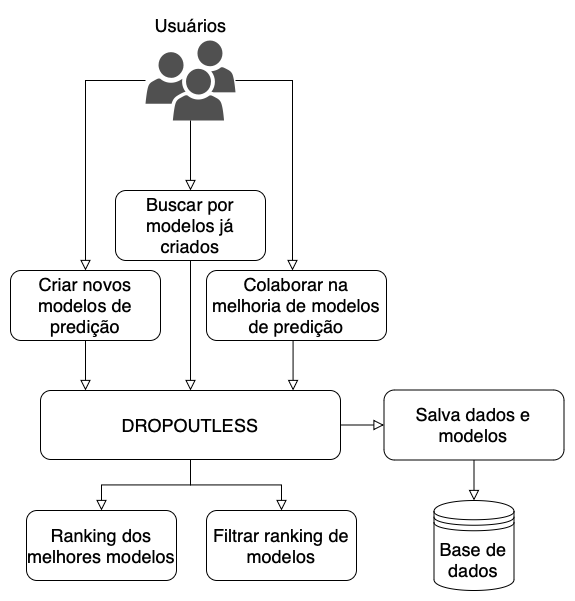
\includegraphics[width=0.5\textwidth]{images/contexto.png}
\caption{Diagrama de contexto do sistema Dropoutless.}
\label{fig:contexto}
\end{figure}

O diagrama da Figura \ref{fig:contexto} é uma representação do contexto geral da ferramenta, fornecendo uma visão das responsabilidades do sistema e como ele interage com os usuários e a base de dados. É possível perceber que o sistema permite ao usuário interagir com a criação de modelos de predição, desde a criação do seu próprio modelo até a busca por modelos desenvolvidos por outros usuários e aperfeiçoados pela comunidade de forma colaborativa. Então, o sistema Dropoutless conta com sua principal funcionalidade: 

\begin{itemize}
    \item \textbf{Geração de modelos de predição com o uso da tecnologia AutoML}: descrito na Seção \ref{sec:Modelo de predição de evasão}, essa funcionalidade possibilita ao usuário criar e treinar novos modelos de predição, se adaptando ao conjunto de dados que o mesmo possuir, ou ainda, utilizar um modelo pronto, previamente treinado em conjuntos de dados de outros usuários.
\end{itemize}



% Esse  trabalho,  conforme  fundamentado,  baseia-se  no  conceito  do  Modelo  3Cde  colaborac ̧ ̃ao.    Segundo  fuks,  o  Modelo  3C  analisa  colaborac ̧ ̃ao  em  3  dimens ̃oes:comunicac ̧ ̃ao, coordenac ̧ ̃ao e cooperac ̧ ̃ao.  A comunicac ̧ ̃ao, caracteriza-se pela troca demensagens, a coordenac ̧ ̃ao pelo gerenciamento de pessoas e a cooperac ̧ ̃ao pela atuac ̧ ̃aoconjunta no espac ̧o compartilhado.Assim sendo, relaciona a ferramenta delineada com o Modelo 3C de colaborac ̧ ̃aopor interm ́edio da seguinte configurac ̧ ̃ao: a Coordenac ̧ ̃ao ́e realizada por Usu ́arios Admi-nistradores.  Esses usu ́arios disp ̃oem de maior grau na hierarquia dentro da ferramenta,logo,  possuem responsabilidades,  tais como:  coordenar tanto novas entradas de dadosquanto dados j ́a aprovados na ferramenta; coordenar Usu ́arios N ̃ao Registrados e Colabo-radores e controlar a comunicac ̧ ̃ao entre esses. Essas atividades trar ̃ao mais confiabilidadepara os dados presentes e dificultar ́a ac ̧ ̃oes de usu ́arios com m ́as intenc ̧ ̃oes.A comunicac ̧ ̃ao ser ́a realizada de forma ass ́ıncrona por meio dofeedbackdas ac ̧ ̃oesdo Usu ́ario Colaborador dentro da ferramenta, isso atrav ́es das avaliac ̧ ̃oes dos sinais, cri-ados  por  tais  colaboradores,  pelos  Usu ́arios  N ̃ao  Registrados.   J ́a  a  cooperac ̧ ̃ao  ser ́a  oregistro de todas formas de comunicac ̧ ̃ao coordenadas pelos Usu ́arios Administradoresem um espac ̧o compartilhado, possibilitando que todos os usu ́arios consigam obter estasinformac ̧ ̃oes e as utilizem como forma de aprendizado em Libras.

% Os requisitos para a criação da Minuta Colaborativa foram baseados no Modelo 3C de Colaboração[Fucks et al., 2011]. Tendo em vista que a população iria atuar em uma  página com  uma  minuta partilhada (cooperar),  iriam  se  comunicar  através  de comentários (comunicar) e iriam comentar diferentes tipos de itens e seções da minuta, com a necessidade de autenticação, deforma coordenada

% O Modelo 3C de Colaboração analisa a colaboração em três dimensões: comunicação, coor- denação e cooperação. A comunicação é caracterizada pela troca de mensagens, pela argu- mentação e pela negociação entre pessoas; a coordenação é caracterizada pelo gerenciamento de pessoas, atividades e recursos; e a cooperação é caracterizada pela atuação conjunta no espaço compartilhado para a produção de objetos ou informações.

A forma como a colaboração ocorre no sistema Dropoutless se baseia no Modelo 3C de Colaboração, que analisa a colaboração em três dimensões: a comunicação, a coordenação e a cooperação \cite{fuks2011teorias}. A dimensão da comunicação é a ação de troca de mensagens para que haja o entendimento comum entre os envolvidos, podendo ser feita de forma síncrona ou assíncrona. A coordenação é o elemento que organiza e coordena as ações e demandas geradas pela comunicação, é a dimensão que mantém a ordem no espaço compartilhado. Por fim, a dimensão da cooperação é onde todas as partes envolvidas trabalham juntas em uma atividade no espaço compartilhado.

Sendo assim, essas dimensões podem ser vistas no Dropoutless, no qual a comunicação entre usuários (prevista como trabalho futuro) ocorrerá através do compartilhamento de materiais  dos comentários existentes nas publicações, em que os professores poderiam escrever suas opiniões sobre o conteúdo postado. A coordenação, que é definida como o gerenciamento de pessoas e recursos, pode ser vista na plataforma através dos usuários moderadores, que possuem os privilégios de agir de forma a moderar o conteúdo, tendo o poder de apagar modelos e excluir contas de usuários por mau uso da ferramenta. Por fim, a cooperação ocorre na criação de modelos de predição através do compartilhamento de dados com a plataforma, o que permite que o modelo treine com cada vez mais dados de diferentes contextos, podendo gerar uma melhoria nas predições geradas.

\section{Cenário de uso}
\label{sec:Cenário de uso}
Esta seção tem como objetivo apresentar um cenário de uso da plataforma Dropoutless, com objetivo de analisar a viabilidade da solução e demonstrar como ela pode ser usada para prever a evasão de forma colaborativa.

A Figuras \ref{fig:criarmodelo} e \ref{fig:prever} apresentam as principais telas do sistema Dropoutless. Além delas, há ainda a tela de Login, a página inicial onde é apresentado uma descrição da ferramenta e como o usuário pode utilizá-la, a tela de ranking de modelos e a tela de gerenciamento dos modelos criados e salvos. 

\begin{figure}
\centering
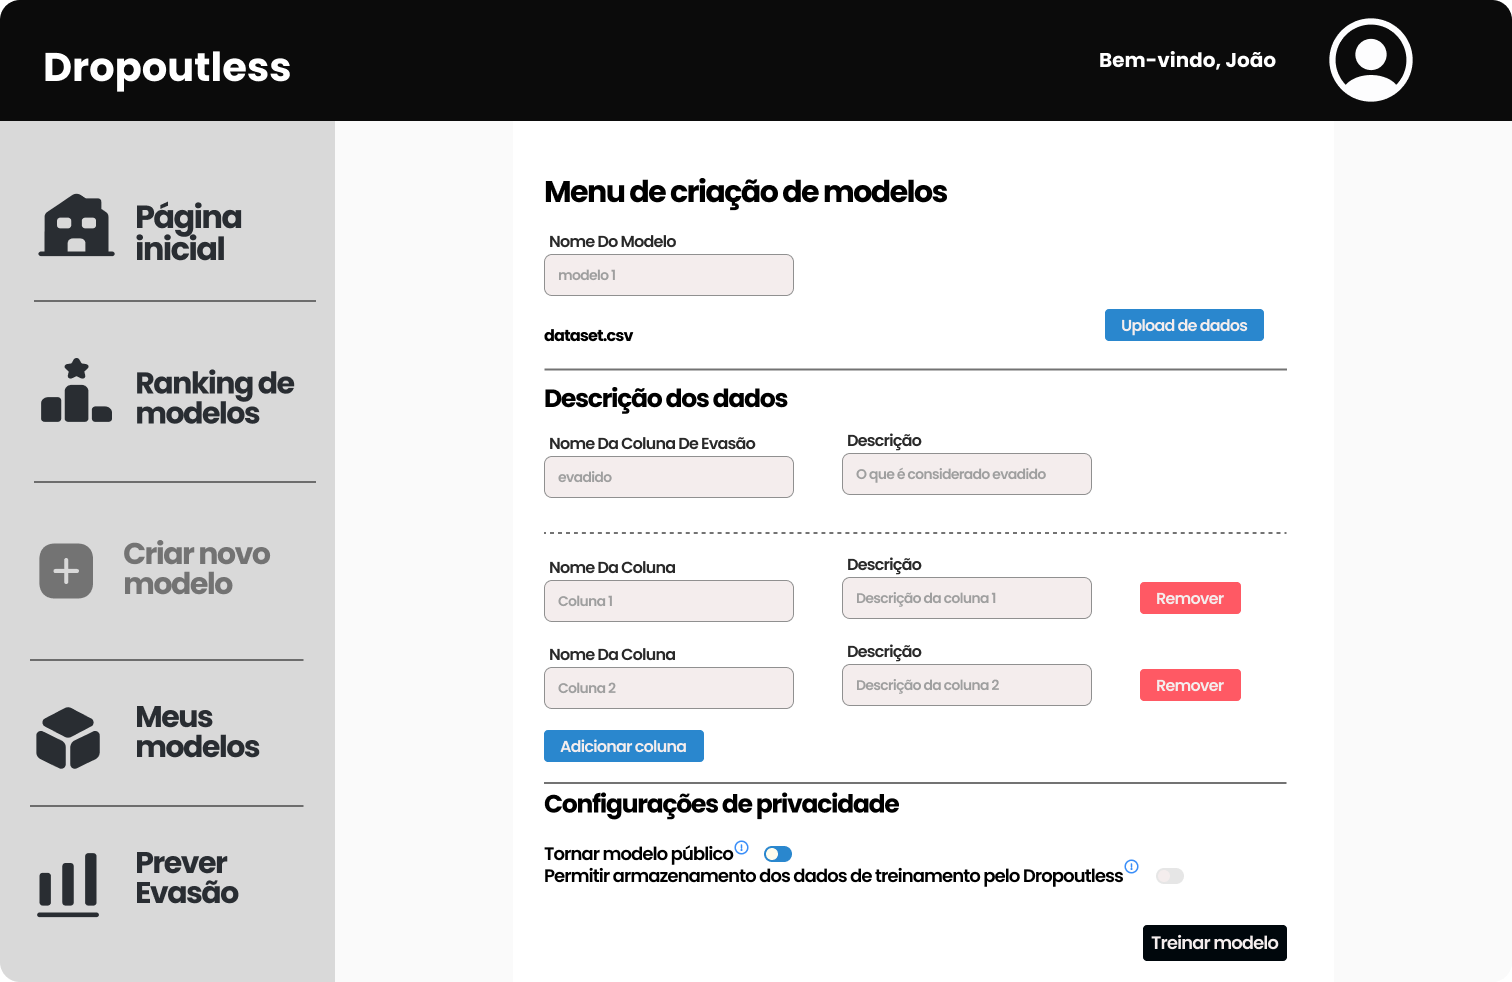
\includegraphics[width=0.7\textwidth]{images/criar modelo.png}
\caption{Tela de criação de modelos do sistema Dropoutless.}
\label{fig:criarmodelo}
\end{figure}

Para apresentar um caso de uso do Dropoutless, o usuário ``João" é utilizado como exemplo. ``João" é um professor do curso de Ciência da Computação, que leciona a disciplina de Algoritmos. Todos os semestre, ``João" percebe estudantes que abandonaram a disciplina por diferentes motivos, desde faltas excessivas até notas baixas em provas. Visando reduzir a evasão das turmas de sua disciplina, ``João" decide utilizar a ferramenta Dropoutless para identificar estudantes que possam evadir com antecedência e poder tomar ações para evitar isso.

Então, ``João" realiza o cadastro na plataforma, clicando no link para criar uma conta na tela de login. De posse de uma conta, ``João" seleciona a opção de criar um modelo, onde determina um nome para o seu modelo, faz o carregamento dos dados que coletou sobre sua turma e preenche o nome e descrição de todas as colunas presentes no arquivo do tipo \textit{comma separated values} (CSV) selecionado. ``João" optou por usar como dados as notas na primeira prova, a frequência dos estudantes e a entrega do primeiro trabalho, embora a ferramenta aceite quaisquer outros dados sobre provas, trabalhos, frequência, participação, entre outros. Nesta tela, ``João" pode escolher se deseja compartilhar seu modelo para que outros usuários possam utilizá-lo para realizar predições sobre os dados que possuem. Por fim, clicando no botão "Treinar modelo" as configurações e arquivos são enviados para que o AutoML realize a criação e treinamento do modelo.

\begin{figure}
\centering
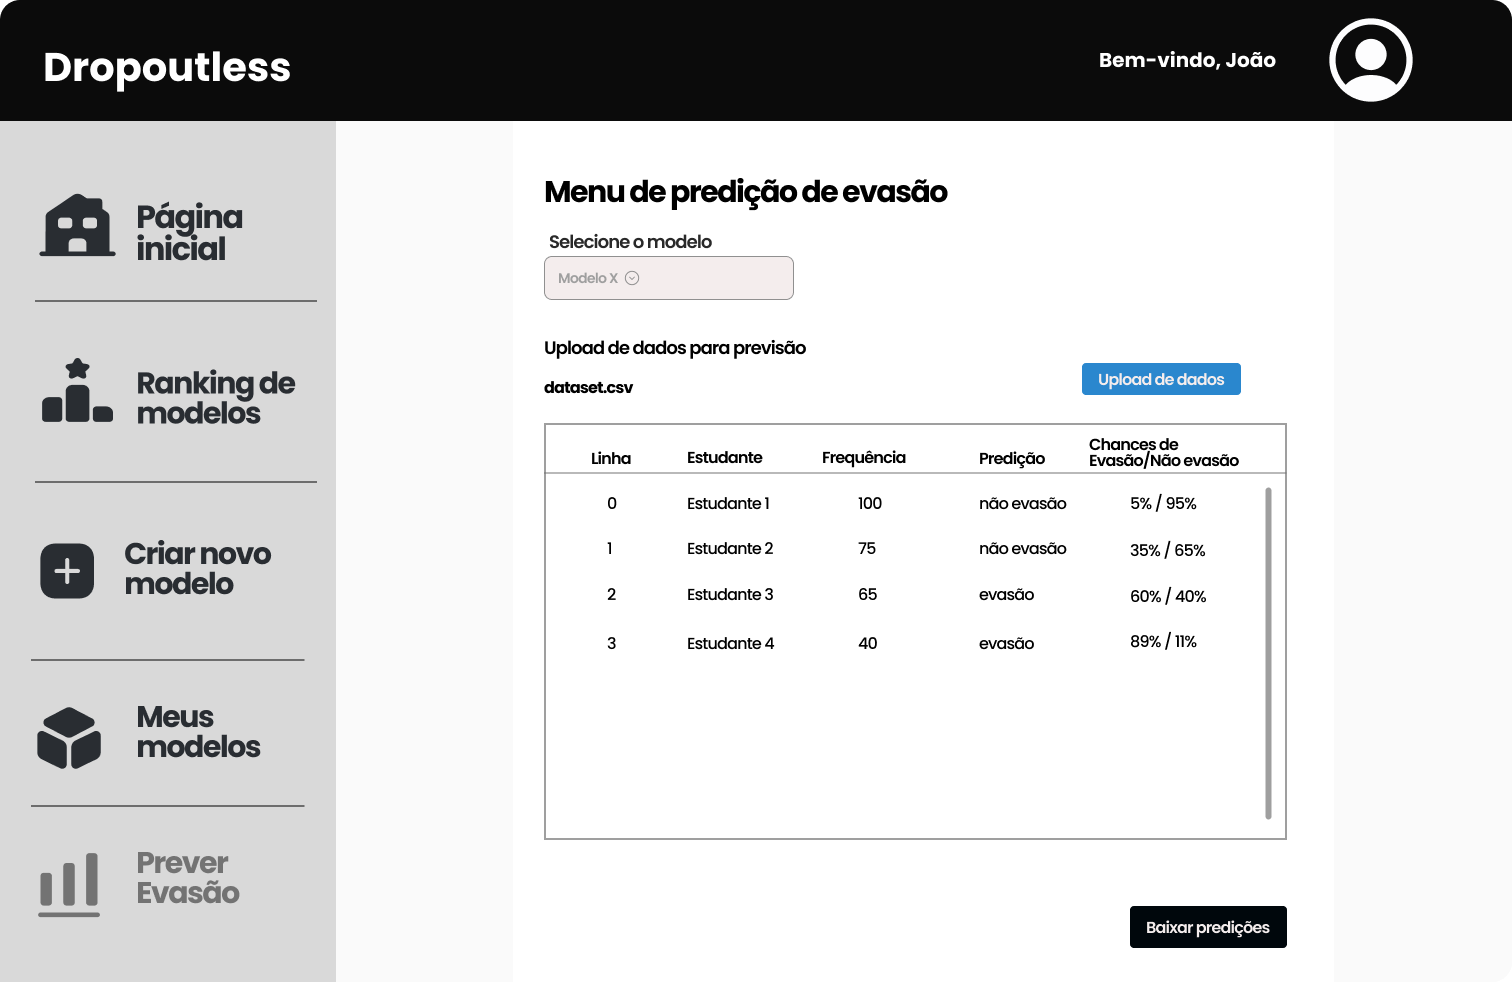
\includegraphics[width=0.7\textwidth]{images/prever.png}
\caption{Tela de predição de evasão do sistema Dropoutless.}
\label{fig:prever}
\end{figure}

Quando o modelo estiver pronto, ``João" poderá visualizá-lo na tela da Figura \ref{fig:prever}. Nesta tela, ``João" deve fornecer os dados atuais dos estudantes dos quais deseja prever as chances de evasão, podendo observá-las na própria plataforma ou ainda baixar um arquivo CSV com os resultados.

Porém, devido a baixa quantidade de dados disponibilizados para o treinamento, visto que ``João" apenas apresentou os dados da turma anterior, o modelo desenvolvido obteve um baixo desempenho. Então, para mitigar esse problema, ``João" buscou no ranking de modelos por um que possuísse métricas de desempenho melhores e que utilizasse na predição a ``Nota de Prova" e a ``Frequência", conforme evidenciado nas \textit{tags}. Para identificar quais métricas ele gostaria de maximizar na busca por um modelo, ``João" pôde ler a explicação sobre o que cada uma delas representa, já que a explicação aparece ao passar o cursor em cima do ícone de informações. Com isso, ``João" selecionou o melhor modelo e salvou ele clicando no coração para curtir. 

Por fim, ``João" realiza novas predições com o modelo salvo e verifica um estudante com altas chances de evasão. Determinado a ajudar esse estudante a concluir a disciplina de algoritmos, ``João" desenvolve atividades extras para engajar o estudante e consegue impedir uma possível evasão.

O caso de uso de ``João" apresentou como o usuário pode interagir com a plataforma e participar ativamente dela criando novos modelos de predição. Com isso, é possível perceber os benefícios que a criação de um sistema colaborativo pode trazer para o problema da evasão.

\section{Arquitetura da plataforma}
\label{sec:Arquitetura da plataforma}

A Figura \ref{fig:arquitetura} apresenta a arquitetura do sistema Dropoutless, cuja base é de uma arquitetura de microsserviços. Nela é possível ver a divisão de cada parte da estrutura, onde o usuário interage com o \textit{Frontend}, a parte gráfica da aplicação que funcionará na \textit{Web}, e esta se comunica com as demais interfaces de programação de aplicações (APIs) para realizar as funções necessárias de forma desacoplada. As APIs se comunicam com um banco de dados único, responsável por armazenar as informações de postagem dos usuários, modelos criados e dados de criação de novos usuários.

\begin{figure}[ht]
\centering
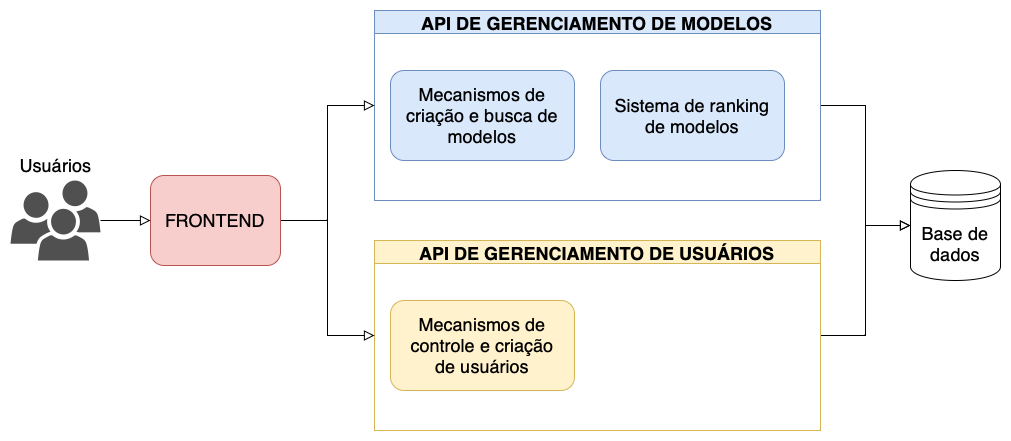
\includegraphics[width=0.8\textwidth]{images/arquitetura.png}
\caption{Representação gráfica da arquitetura do Dropoutless.}
\label{fig:arquitetura}
\end{figure}
% adicionar nota de rodapé explicando o autogluon

A API de gerenciamento de modelos é responsável por duas funções principais, a primeira é a de fornecer os meios de criação, busca e gerenciamento de modelos criados utilizando a biblioteca de AutoML, o Autogluon. Com isso, esse módulo fornecerá um canal de comunicação que permite criar novos modelos utilizando arquivos no formato CSV. Já o módulo de \textit{ranking} de modelos será responsável pela organização dos mesmos de acordo com os filtros selecionados pelo usuário. O \textit{ranking} determina quais são os melhores preditores baseando-se em métricas fornecidas pela biblioteca, como por exemplo a acurácia do modelo. Esta API também realiza o fluxo presente no diagrama da Figura \ref{fig:fluxograma}, onde ocorre a melhoria contínua dos modelos de predição através de seu uso por novos usuários. Além do armazenamento do modelo treinado com os novos dados, no caso de melhora de desempenho em relação ao anterior, também é de responsabilidade desta API realizar os procedimentos para garantir a anonimização dos dados para o armazenamento na base de dados.

O modelo mostra no ranking apenas os modelos que satisfazem os filtros fornecidos pelo usuário, como por exemplo, levar em consideração a quantidade de faltas do estudante para a predição, então nesse caso o ranking contaria apenas com modelos que usam dessa informação para a tomada de decisão.

\begin{figure}[ht]
\centering
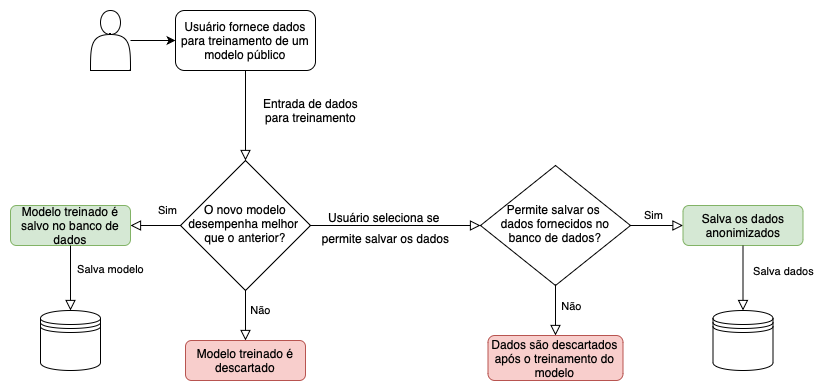
\includegraphics[width=0.9\textwidth]{images/fluxograma.png}
\caption{Fluxo da melhoria contínua de modelos.}
\label{fig:fluxograma}
\end{figure}

% AQUI COLOCAR A PARTE DE SALVAR OS DADOS SAINDO DO MODELO MELHOR DESEMPENHO

Então, para o funcionamento de todas as partes, a API de gerenciamento de usuários é necessária, visto que ela é a responsável pelo cadastro e login daqueles que utilizam a ferramenta. Além disso, essa API gerencia os dados como nome, email, foto de perfil e senha que o usuário preenche na plataforma.

\subsection{Modelo de predição de evasão}
\label{sec:Modelo de predição de evasão}

Diante da natureza do problema, os usuários que não são familiarizados com aprendizado de máquina utilizariam o sistema, portanto, é fundamental que a ferramenta possa realizar o máximo possível de processos de forma automatizada, de modo que o usuário leigo não precise entender o funcionamento do mesmo para gerar seu modelo. Por conta disso, a ferramenta Dropoutless emprega o uso de técnicas de AutoML para tal. 

Segundo a AutoML\footnote{https://www.automl.org/automl/}, o \textit{Machine Learning} automatizado pode ser pensado como um algoritmo de busca especializado em achar soluções ótimas para cada componente do pipeline de ML. Com isso, ele permite a automatização de processos chaves como a engenharia de \textit{features}, o pré-processamento de dados e a otimização de hiperparâmetros na busca pelo melhor modelo.

Como a predição de evasão dinâmica e simples é o foco principal da ferramenta Dropoutless, então, a biblioteca de AutoML escolhida para o sistema é a Autogluon\footnote{https://auto.gluon.ai/stable/index.html}, por se tratar de uma ferramenta \textit{open-source} e gratuita, além de declarar, em sua documentação, que realiza os processo de limpeza e preparação dos dados, o que diminui a necessidade do usuário de entender certos conceitos para usar a ferramenta. No mais, a escolha de uso da tecnologia AutoML agrega na forma de trabalho de um sistema colaborativo, visto que os usuários poderão colaborar dentro da plataforma na criação de modelos de ML cada vez melhores através do compartilhamento dos dados, contribuindo também para a redução de escassez dos mesmos, já que um único modelo poderia contar com informações de estudantes de disciplinas diversas de diferentes professores.

\section{Implicações Éticas}
\label{sec:implicaoes éticas}

Quando se armazena e manipula dados dos usuários, como o Dropoutless faz, deve-se ter precauções para garantir a privacidade de todas as partes. Sendo assim, é imprescindível à ferramenta a determinação de processos para lidar com a anonimização dos dados dos estudantes, visto que o objetivo dela é que o usuário possa usar os dados reais de suas turmas para gerar as previsões. Então, para lidar com essa situação, a ferramenta apresenta indicações de como tornar os dados anônimos antes de realizar o carregamento dos mesmos, através de ícone explicativos na tela de criação de modelo. Além disso, quando o usuário dá a permissão de armazenamento desses dados para treinamentos futuros de modelos, a API de gerenciamento dos modelos realiza a limpeza desses dados, transformando variáveis de texto em categorias numéricas através de técnicas como \textit{One Hot Encoder} e \textit{Label Encoder}, para impedir o armazenamento do nome dos estudantes.

Outra situação que se deve observar ao lidar com ML, em especial aquelas que fazem classificações de pessoas, nesse caso como evasão ou não evasão, é que as classificações podem muitas vezes estar erradas. Então, o usuário que agir com base na classificação dada pelo modelo, deve ter em mente que o mesmo pode estar incorreto. Para amenizar possíveis tomadas de decisões mais drásticas influenciadas pelos resultados do modelo, o mesmo apresenta as porcentagens de chance do estudante evadir ou não evadir, demonstrando que não há certeza nas respostas, apenas há uma chance maior de um fenômeno acontecer em detrimento do outro.


\section{Conclusões e Trabalhos Futuros}
\label{sec:conclusão}

Este artigo teve como principal objetivo o desenvolvimento de uma ferramenta colaborativa de predição de evasão em disciplinas. Observou-se que os trabalhos envolvendo predição de evasão tendem a focar na evasão em cursos e com modelos de ML pré-desenvolvidos, o que torna a ferramenta Dropoutless um diferencial por seu foco na evasão em disciplinas e uso de AutoML em um sistema colaborativo para a melhora contínua das predições.

Como trabalhos futuros, podem ser citadas algumas melhorias na plataforma, como o estudo da otimização dos hiperparâmetros fornecidos para os algoritmos do AutoML, com o objetivo de obter desempenhos melhores nos modelos. Além disso, pode ser acrescentado um módulo de compartilhamento de materiais com o objetivo de permitir ao usuário publicar textos e arquivos que descrevem métodos de redução da evasão testados por ele. Além das melhorias na plataforma, ressalta-se a necessidade de testar a plataforma com usuários e dados reais, para verificar a eficiência da solução em um ambiente colaborativo.

\bibliographystyle{sbc}
\bibliography{sbc-template}

\end{document}
